\section{Durchführung}

\begin{figure}[H]
    \centering
    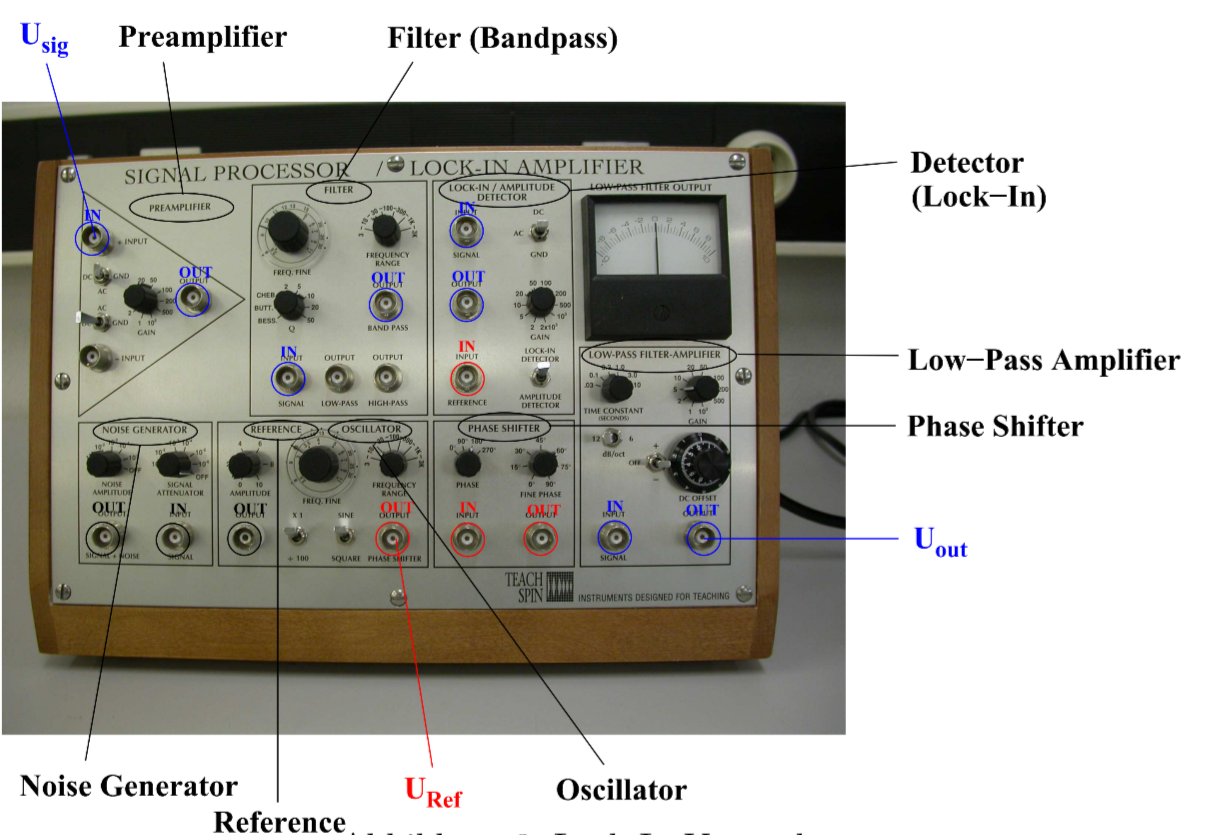
\includegraphics{Bilder/LockIn.png}
    \caption{Aufbau des Lock-In Verstärkers.\cite{V303}}
    \label{fig:LockIn}
\end{figure}
\begin{figure}[H]
    \centering
    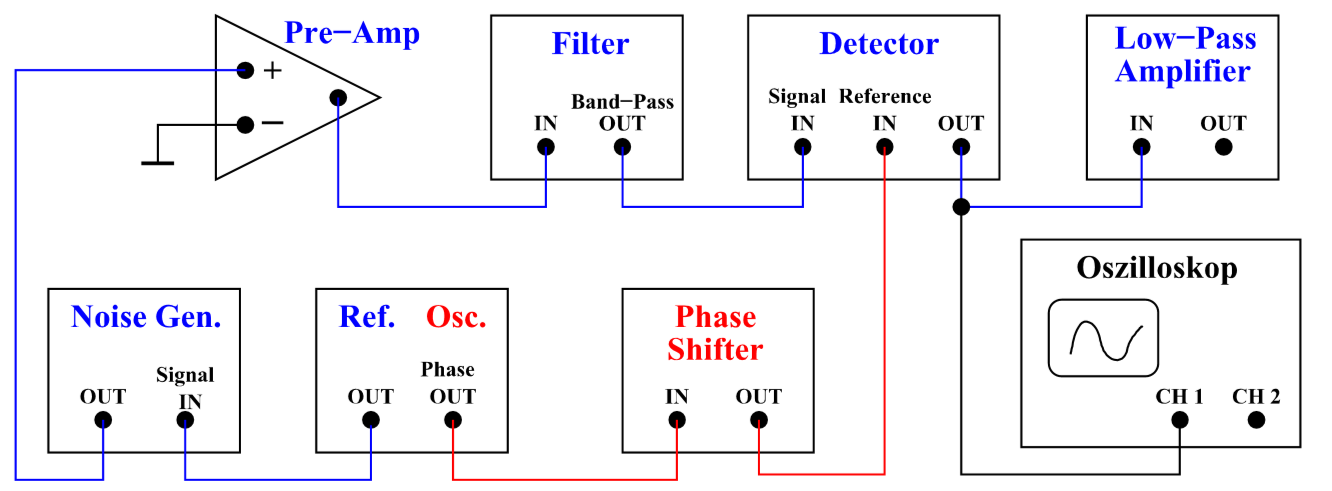
\includegraphics{Bilder/LockInShema.png}
    \caption{Schematischer Aufbau der Lock-In Verstärkers. \cite{V303}}
    \label{fig:LockInSchema}
\end{figure}

\noindent 
Zunächst wird für den Lock-In-Verstärker, abgebildet in Abbildung \ref{fig:LockIn}, festgestellt, dass die Oszillatorspannung einen konstanten Wert von $\qty{3,245}{\volt}$ annimmt.
Danach wird der Lock-In Verstärker wie in Abb \ref{fig:LockInSchema} verkabelt, wobei der Noise Generator zunächst ausgeschaltet bleibt.
Für die Oszillatorspannung wird eine Sinusspannung mit einer Amplitude von $\qty{10}{\milli\volt}$ und einer Frequenz von 
$\qty{1}{\kilo\hertz}$. Als Referenzspannung wird ebenfalls eine Sinusspannung mit der gleichen Frequenz angelegt. Diese überlagert
die Oszillatorspannung, was am Oszilloskop sichtbar wird. Die Spannungverläufe für verschiedene Phasenverschiebungen der Referenzspannung
werden dann festgehalten und die Amplitude der Ausgangspannung notiert. Die selbe Messung wird dann mit einer Störung, die 
von dem Noise Generator verursacht wird wiederholt. \\

\noindent Als nächstes wird der Noisegenerator durch eine Photodetektorschaltung wie in Abbildung \ref{fig:photo} ersetzt.
\begin{figure}[H]
    \centering
    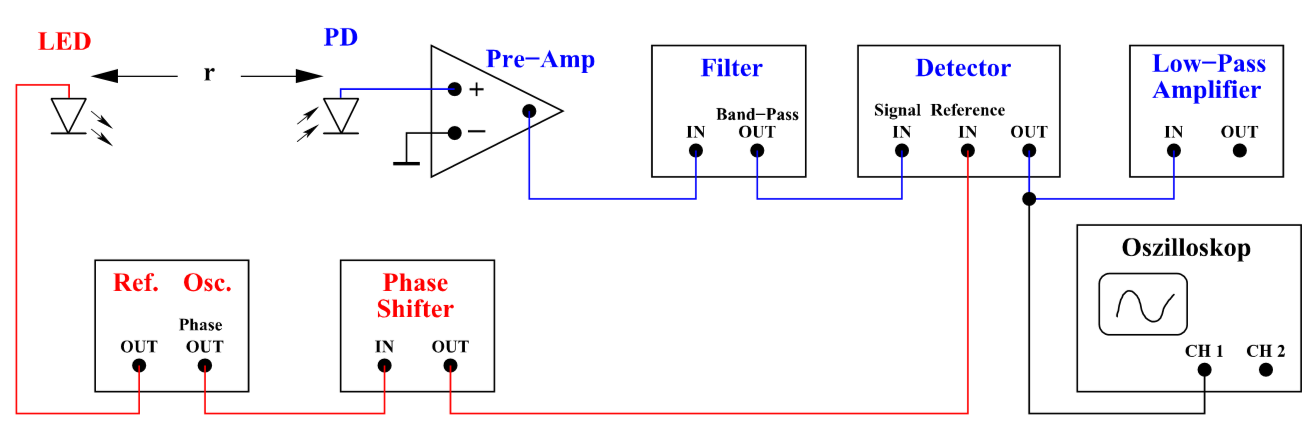
\includegraphics{Bilder/PhotoLockInn}
    \caption{Schematischer Aufbau des Lock-Inn Verstärkers mit Photodetektor. \cite{V303}}
    \label{fig:photo}
\end{figure}
Der von der Oszillatorspannung erzeugte LED erzeugt im Detektor dann eine der Oszillatorspannung entsprechende Spannung, die 
allerdings gestört wurde. Hier wird dann die Ausgangspannung gegen den Abstand $r$ aufgetragen.

\label{sec:Durchführung}
